\chapter{Divergences and Dual Norms}

\index{dual!norm}% strictindex
\label{sec-divergences-dual-norms}


This chapter compares OT with divergence-based and adversarial ways of measuring discrepancy. The main stake is topological: $\phi$-divergences are cheap but strong, while dual norms and GAN objectives can be weak enough to compare singular measures. The discussion connects classical information divergences~\cite{ciszar1967information,ali1966general} with modern integral probability metrics and generative modeling~\cite{sriperumbudur2009integral,GAN,WassersteinGAN}.
\index{generative model}% strictindex
\index{integral probability metric}% strictindex
\index{phi-divergence}% strictindex
\index{dual!norm}% strictindex

%%%%%%%%%%%%%%%%%%%%%%%%%%%%%%%%%%%%%%%%%%%%%%%%%%%%%%%%%%%%%%%%%%%%%%%%
\section{Dual norms (Integral Probability Metrics)}
\index{dual!norm}% strictindex
\index{integral probability metric}% strictindex
\label{sec-dual-norms}

Dual norms generalize the $\Wass_1$ test-function principle. They are useful in statistics because they compare distributions by restricting the discriminator class.
\index{discriminator class}% strictindex
\index{dual!norm}% strictindex

\paragraph{Integral probability metrics.}
\index{integral probability metric}% strictindex

Formulation~\eqref{eq-w1-cont} is a special case of a dual norm. This viewpoint designs ``weak'' discrepancies by testing signed differences of measures against a controlled class of functions.
\index{measurable function}% strictindex
\index{dual!norm}% strictindex

\begin{defn}[Dual norm and integral probability metric]\label{def-dual-norm-ipm}
\index{dual!norm}% strictindex
\index{integral probability metric}% strictindex
	For a symmetric convex set $B$ of measurable functions, define on signed measures $\xi$
	\eql{\label{eq-dual-norm-cont}
		\norm{\xi}_B \eqdef
		\usup{\f} \enscond{ \int_{\X} \f(x) \d\xi(x) }{ \f \in B}.
	}
	When this quantity is applied to $\al-\be$ for probability measures, it is often called an integral probability metric.
\end{defn}
The choice of the test-function class $B$ determines both the topology and the statistical behavior of the discrepancy; see~\cite{sriperumbudur2012empirical,sriperumbudur2009integral,sriperumbudur2008injective}.
\index{integral probability metric}% strictindex
\index{dual!norm}% strictindex

\begin{example}[Total variation]
\index{total variation}% strictindex
As recalled in Definition~\ref{defn-total-variation} and Proposition~\ref{prop-tv-dual-measure}, total variation is the dual norm associated with the unit ball of continuous functions
\eq{
	B = \enscond{f \in \Cc(\X)}{\norm{f}_\infty \leq 1}.
}
Total variation is the canonical nontrivial example of a discrepancy that is both a $\phi$-divergence and a dual norm; see~\cite{sriperumbudur2009integral}.
\index{total variation}% strictindex
\index{phi-divergence}% strictindex
\index{dual!norm}% strictindex
\end{example}

\begin{example}[$\Wass_1$ norm]
$\Wass_1$, as defined in~\eqref{eq-w1-cont}, is the dual norm~\eqref{eq-dual-norm-cont} associated with
\index{dual!norm}% strictindex
\eq{
	B = \enscond{f}{\Lip(f) \leq 1}
}
the set of 1-Lipschitz functions.
\index{Lipschitz!function}% strictindex
\end{example}

\begin{example}[Flat norm and Dudley metric]
\index{norm!flat}% strictindex
\index{Dudley metric}% strictindex
If the set $B$ is bounded and separates measures, then $\norm{\cdot}_B$ is a norm on the whole space $\Mm(\Xx)$ of finite measures.
\index{finite measure}% strictindex
%
	This is not the case of $\Wass_1$, which is only finite on signed measures $\xi$ such that $\int_\X \d\xi=0$; otherwise $\norm{\xi}_B=+\infty$ because constants belong to the Lipschitz ball.
%
This is remedied by imposing a bound on the value of the potential $\f$, which leads for instance to the flat norm,
\index{norm!flat}% strictindex

\eql{\label{eq-set-flatnorm}
	B=\enscond{f}{\Lip(f) \leq 1 \qandq \norm{\f}_\infty \leq 1}.
}
On compact metric spaces, it metrizes weak convergence on the whole space $\Mm(\X)$ of finite measures.
\index{finite measure}% strictindex
\index{weak!convergence}% strictindex
%
The finite-dimensional version is obtained from the usual $\Wass_1$ dual linear program by adding the box constraints $\abs{\fD_k}\leq1$.
%
The flat norm is sometimes called the ``Kantorovich--Rubinstein'' norm~\cite{hanin1992kantorovich} and has been used as a fidelity term for inverse problems in imaging~\cite{lellmann2014imaging}.
\index{norm!flat}% strictindex
%
The flat norm is similar to the Dudley metric, which uses
\index{Dudley metric}% strictindex
\eq{\label{eq-set-dudley}
	B=\enscond{f}{\norm{\nabla \f}_\infty + \norm{\f}_\infty \leq 1}.
}
\end{example}

\begin{figure}[ht]
\centering
\setlength{\tabcolsep}{2pt}
\begin{tabular}{@{}ccc@{}}
\small $\Wass_1$ witness & \small MMD witness & \small total variation witness \\[-.15em]
\index{total variation}% strictindex
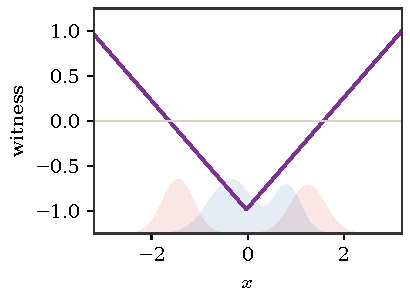
\includegraphics[width=.31\linewidth]{figures/dualnorms-ipm-witnesses--w1.pdf} &
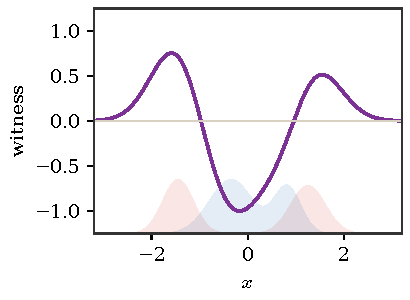
\includegraphics[width=.31\linewidth]{figures/dualnorms-ipm-witnesses--mmd.pdf} &
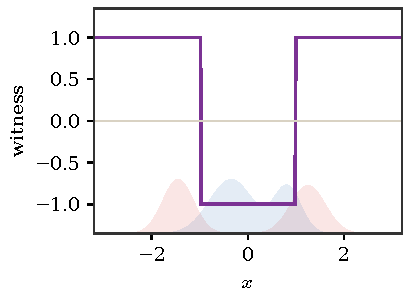
\includegraphics[width=.31\linewidth]{figures/dualnorms-ipm-witnesses--tv.pdf}
\end{tabular}
\caption{Dual witnesses for integral probability metrics. The red and blue curves are two one-dimensional probability densities and the violet curve is a normalized optimal dual witness $f^\star_{\alpha,\beta}$ for the IPM variational problem~\eqref{eq-dual-norm-cont}. $\Wass_1$ restricts the slope through Kantorovich--Rubinstein duality~\eqref{eq-w1-cont}, MMD restricts the RKHS norm as in Proposition~\ref{prop-kernel-rkhs-dual}, and total variation can saturate pointwise and therefore reacts sharply to signed density differences.}
\index{Kantorovich-Rubinstein!duality}% strictindex
\index{integral probability metric}% strictindex
\index{total variation}% strictindex
\index{dual!norm}% strictindex
\index{RKHS}% strictindex
\label{fig:dualnorms-ipm-witnesses}
\end{figure}

The following proposition gives a useful compact-space criterion. The dual ball should be rich enough to approximate continuous observables, but compact enough for weak convergence to imply uniform convergence over the discriminator class.
\index{discriminator class}% strictindex
\index{weak!convergence}% strictindex

\begin{prop}[Metrization by dual norms]\label{prop-dual-norm-metrization}
\index{dual!norm}% strictindex
	Assume that $\Xx$ is compact, that $B=-B$, and that the measures considered are probability measures.
\index{probability measure}% strictindex
	\begin{enumerate}
		\item If every function in $\Cc(\Xx)$ can be uniformly approximated by elements of $\Span(B)$, then $\norm{\al_n-\al}_B \rightarrow 0$ implies $\al_n \rightharpoonup \al$.
		\item If $B \subset \Cc(\Xx)$ is compact for $\norm{\cdot}_\infty$, then $\al_n \rightharpoonup \al$ implies $\norm{\al_n-\al}_B \rightarrow 0$.
	\end{enumerate}
\end{prop}
\begin{proof}
	For the first implication, $\norm{\al_n-\al}_B\to0$ and the symmetry of $B$ imply
	\[
		\abs{\dotp{f}{\al_n-\al}}\leq \norm{\al_n-\al}_B
		\qforq f\in B.
	\]
	By linearity, integrals converge for every $h\in\Span(B)$. Let $u\in\Cc(\Xx)$ and choose $h\in\Span(B)$ with $\norm{u-h}_\infty\leq\eta$. Since $\al_n$ and $\al$ are probabilities,
	\[
		\abs{\dotp{u}{\al_n-\al}}
		\leq
		\abs{\dotp{h}{\al_n-\al}}+2\eta.
	\]
	Taking the limsup as $n\to\infty$ and then letting $\eta\to0$ gives $\dotp{u}{\al_n}\to\dotp{u}{\al}$ for all $u\in\Cc(\Xx)$, which is weak convergence.
\index{weak!convergence}% strictindex

	For the second implication, assume $\al_n\rightharpoonup\al$ and choose a subsequence $(\al_{n_k})_k$ such that $\norm{\al_{n_k}-\al}_B\to\limsup_n\norm{\al_n-\al}_B$. Since $B$ is compact and the map $f\mapsto\dotp{f}{\al_{n_k}-\al}$ is continuous on $B$, the supremum is attained by some $f_{n_k}\in B$. Extracting a further subsequence if needed, $f_{n_k}\to f$ uniformly for some $f\in B$. Then
	\[
		\dotp{f_{n_k}}{\al_{n_k}-\al}
		=
		\dotp{f}{\al_{n_k}-\al}
		+\dotp{f_{n_k}-f}{\al_{n_k}}
		-\dotp{f_{n_k}-f}{\al}.
	\]
	The first term tends to zero by weak convergence and the last two by uniform convergence. Hence every limsup subsequence has limit zero, proving $\norm{\al_n-\al}_B\to0$.
\index{weak!convergence}% strictindex
\end{proof}

\begin{cor}[Wasserstein metrizes weak convergence]\label{cor-topol-wass}
	On a compact metric space, $\Wass_p$ metrizes weak convergence on probability measures for every $p\geq1$.
\index{probability measure}% strictindex
\index{weak!convergence}% strictindex
\end{cor}
\begin{proof}
	For $p=1$, take $B=\enscond{f}{\Lip(f)\leq1}$. The span of $B$ contains all Lipschitz functions, and Lipschitz functions are dense in $\Cc(\Xx)$ on compact metric spaces. This gives the implication $\Wass_1(\al_n,\al)\to0\Rightarrow \al_n\rightharpoonup\al$ by Proposition~\ref{prop-dual-norm-metrization}.
\index{Lipschitz!function}% strictindex
\index{dual!norm}% strictindex

	Conversely, constants do not change the pairing with $\al_n-\al$. Fix $x_0\in\Xx$ and normalize potentials by $f(x_0)=0$. The normalized unit Lipschitz ball is uniformly bounded by $\mathrm{diam}(\Xx)$ and equicontinuous, hence compact in $\norm{\cdot}_\infty$ by Arzel\`a--Ascoli. Proposition~\ref{prop-dual-norm-metrization} gives $\Wass_1(\al_n,\al)\to0$. Proposition~\ref{prop-comp-wass-p} shows that all $\Wass_p$ distances induce the same topology on a compact space, so the result follows for every $p\geq1$.
\end{proof}

\section{Dual RKHS Norms and Maximum Mean Discrepancies}
\index{maximum mean discrepancy}% strictindex
\index{RKHS}% strictindex
\label{sec-rkhs-mmd}

Kernel methods turn probability measures into mean elements of a reproducing kernel Hilbert space (RKHS). The resulting Hilbertian dual norms are quadratic discrepancies, handled with Euclidean geometry while retaining a weak test-function interpretation. We first recall the positivity assumptions under which the quadratic form on signed measures is nonnegative.
\index{probability measure}% strictindex
\index{signed!measure}% strictindex
\index{dual!norm}% strictindex

\begin{defn}[Positive and conditionally positive kernels]\label{def-positive-kernels}
\index{kernel!positive}% strictindex
\index{kernel!conditionally positive}% strictindex
	A symmetric function $\Krkhs:\Xx\times\Xx\to\RR$ is positive definite if for every $n\geq1$, every $x_1,\ldots,x_n\in\Xx$ and every $r\in\RR^n$,
\index{RKHS}% strictindex
	\eql{\label{eq-dual-kern}
		\sum_{i,j=1}^n r_i r_j \Krkhs(x_i,x_j)\geq0.
	}
	It is conditionally positive definite if the same inequality is required only for zero-sum vectors, $\dotp{r}{\ones_n}=0$.
\end{defn}

The conditional version is the right notion for probability distances, because one applies the quadratic form to signed measures $\xi=\al-\be$ of total mass zero. Adding a term of the form $a(x)+a(y)$ to the kernel does not change $\iint \Krkhs(x,y)\d\xi(x)\d\xi(y)$ on such measures, and many natural distance kernels are only conditionally positive definite.
\index{RKHS}% strictindex
\index{signed!measure}% strictindex

\begin{example}[Riesz, energy and Mat\'ern-type kernels]
\index{kernel!Riesz}% strictindex
\index{kernel!energy}% strictindex
\index{kernel!Matern}% strictindex
	On $\RR^d$, translation-invariant kernels are most transparent in Fourier variables. The Riesz family associated with $(-\Delta)^{-s}$ has multiplier $\norm{\om}^{-2s}$ and defines a nonnegative quadratic form on zero-mass measures for which the low-frequency singularity is integrable; this is the kernel counterpart of classical Riesz potentials~\cite{berg84harmonic}. The energy distance corresponds to the conditionally positive kernel $\Krkhs(x,y)=-\norm{x-y}$, whose Fourier multiplier is proportional to $\norm{\om}^{-(d+1)}$; for $\xi=\al-\be$,
\index{kernel!translation-invariant}% strictindex
\index{Riesz potential}% strictindex
\index{Fourier multiplier}% strictindex
\index{kernel!conditionally positive}% strictindex
\index{RKHS}% strictindex
\index{energy!distance}% strictindex
\index{kernel!positive}% strictindex
	\[
		-\iint \norm{x-y}\d\xi(x)\d\xi(y)
	\]
	is the squared energy distance up to a dimensional constant~\cite{schoenberg38,szekely2004testing}.
\index{energy!distance}% strictindex

	Shifted kernels replace $(-\Delta)^{-s}$ by $(-\Delta+\lambda I)^{-s}$ with $\lambda>0$. Their Fourier multiplier $(\norm{\om}^2+\lambda)^{-s}$ is bounded at the origin, hence the kernel is positive definite without imposing zero mass. These are Mat\'ern kernels; in closed form they are radial and involve a modified Bessel function~\cite{wendland2005scattered}. The Laplacian kernel $e^{-\norm{x-y}/\sigma}$ is a low-smoothness Mat\'ern example, while the Gaussian kernel $e^{-\norm{x-y}^2/(2\sigma^2)}$ is the infinite-smoothness limit after the usual rescaling of the Mat\'ern smoothness parameter.
\index{zero mass}% strictindex
\index{Bessel function}% strictindex
\index{kernel!Laplacian}% strictindex
\index{Fourier multiplier}% strictindex
\index{kernel!Gaussian}% strictindex
\index{kernel!Matern}% strictindex
\end{example}

\begin{defn}[Kernel norm and MMD]\label{def-kernel-mmd-norm}
\index{kernel!norm}% strictindex
\index{maximum mean discrepancy}% strictindex
	Let $\Krkhs$ be positive definite. More generally, let $\Krkhs$ be conditionally positive definite and restrict attention to signed measures of total mass zero. For a signed measure $\xi$ with finite kernel energy, the associated norm is
\index{kernel!energy}% strictindex
\index{RKHS}% strictindex
\index{signed!measure}% strictindex
	\eql{\label{eq-kernel-dual}
		\norm{\xi}^2_{\Krkhs}
		\eqdef
		\iint_{\Xx\times\Xx}\Krkhs(x,y)\d\xi(x)\d\xi(y).
	}
	For two probability measures, the maximum mean discrepancy associated with $\Krkhs$ is
\index{probability measure}% strictindex
\index{maximum mean discrepancy}% strictindex
	\[
		\MMD_{\Krkhs}(\al,\be)\eqdef\norm{\al-\be}_{\Krkhs}.
	\]
\end{defn}

These norms are usually called maximum mean discrepancies in statistics and machine learning~\cite{gretton2012kernel,muandet2017kernel}, and kernel norms in shape analysis~\cite{Hofmann2008}. If $X,X'$ are independent with law $\al$, then \(\norm{\al}_{\Krkhs}^2=\EE_{X,X'}(\Krkhs(X,X'))\), whenever this expression is finite.
\index{kernel!norm}% strictindex
\index{RKHS}% strictindex
\index{maximum mean discrepancy}% strictindex

\begin{prop}[Kernel norm as an RKHS dual norm]\label{prop-kernel-rkhs-dual}
\index{dual!norm}% strictindex
\index{RKHS}% strictindex
\index{kernel!norm}% strictindex
\index{norm!RKHS}% strictindex
	Let $\RKHS$ be the RKHS with reproducing kernel $\Krkhs$, and assume that the kernel mean embedding
\index{kernel!mean embedding}% strictindex
	\[
		m_\xi \eqdef \int \Krkhs(x,\cdot)\d\xi(x)
	\]
	is well-defined for the signed measure $\xi$. Then
\index{signed!measure}% strictindex
	\[
		\norm{\xi}_{\Krkhs}
		=
		\sup_{\norm{h}_{\RKHS}\leq1}
		\int h(x)\d\xi(x),
	\]
	so $\norm{\cdot}_{\Krkhs}$ is the dual norm in the sense of~\eqref{eq-dual-norm-cont} associated with the RKHS unit ball.
\index{dual!norm}% strictindex
\end{prop}
\begin{proof}
	By the reproducing property,
	\[
		\int h(x)\d\xi(x)
		=
		\left\langle h,\int \Krkhs(x,\cdot)\d\xi(x)\right\rangle_{\RKHS}
		=
		\langle h,m_\xi\rangle_{\RKHS}.
	\]
	Cauchy--Schwarz gives
	\[
		\sup_{\norm{h}_{\RKHS}\leq1}\int h\d\xi
		=
		\norm{m_\xi}_{\RKHS}.
	\]
	Finally,
	\[
		\norm{m_\xi}_{\RKHS}^2
		=
		\iint \Krkhs(x,y)\d\xi(x)\d\xi(y),
	\]
	which is exactly~\eqref{eq-kernel-dual}.
\end{proof}

\begin{prop}[Universal kernels metrize weak convergence]\label{prop-mmd-metrization}
\index{maximum mean discrepancy}% strictindex
\index{kernel!universal}% strictindex
\index{weak!convergence}% strictindex
	Assume that $\Xx$ is compact and that the RKHS generated by the continuous kernel $\Krkhs$ is dense in $\Cc(\Xx)$ for the uniform norm. Then
\index{RKHS}% strictindex
	\[
		\MMD_{\Krkhs}(\al_n,\al)\to0
		\quad\Longleftrightarrow\quad
		\al_n\rightharpoonup\al
	\]
	for probability measures on $\Xx$.
\index{probability measure}% strictindex
\end{prop}
\begin{proof}
	If $\MMD_{\Krkhs}(\al_n,\al)\to0$, then integrals of all RKHS functions converge. For any $h\in\Cc(\Xx)$ and any $\eta>0$, choose $g\in\RKHS$ with $\norm{h-g}_\infty\leq\eta$. Since $\al_n$ and $\al$ are probabilities,
	\[
		\left|\int h\,\d(\al_n-\al)\right|
		\leq
		2\eta+\left|\int g\,\d(\al_n-\al)\right|,
	\]
	and the last term tends to zero. This proves weak convergence. Conversely, if $\al_n\rightharpoonup\al$, then $\al_n\otimes\al_n$, $\al_n\otimes\al$ and $\al\otimes\al$ converge weakly on the compact product space. Applying this to the continuous bounded function $\Krkhs$ in the identity
\index{weak!convergence}% strictindex
	\[
		\MMD_{\Krkhs}(\al_n,\al)^2
		=
		\iint \Krkhs\,\d\al_n\d\al_n
		-2\iint \Krkhs\,\d\al_n\d\al
		+\iint \Krkhs\,\d\al\d\al
	\]
	gives convergence to zero.
\end{proof}


We refer to~\cite{berlinet03reproducing,Hofmann2008,scholkopf2002learning} for more details on RKHS functional spaces.
\index{RKHS}% strictindex

\begin{rem}[Universal kernels]
\index{kernel!universal}% strictindex
The hypothesis in Proposition~\ref{prop-mmd-metrization} is called universality of the kernel. Equivalently, finite sums of the form $\sum_{i=1}^n a_i \Krkhs(x_i,\cdot)$ are dense in $\Cc(\Xx)$ for the uniform norm. For translation-invariant kernels on $\Xx=\RR^d$, $\Krkhs(x,y)=\Krkhs_0(x-y)$, this is equivalent, in the usual sense on compact sets or with suitable decay assumptions, to the Fourier transform not vanishing on its support~\cite{sriperumbudur2008injective,sriperumbudur2012empirical}.
\index{kernel!translation-invariant}% strictindex
\index{RKHS}% strictindex
\index{maximum mean discrepancy}% strictindex
\end{rem}

In the special case where $\al$ is a discrete measure, one thus has the simple expression
\eq{
	\norm{\al}_{\Krkhs}^2 = \sum_{i=1}^n \sum_{i'=1}^n \a_i\a_{i'} \KrkhsD_{i,i'} = \dotp{\KrkhsD\a}{\a}
\index{RKHS}% strictindex
	\qwhereq
	\KrkhsD_{i,i'} \eqdef \Krkhs(x_i,x_{i'}).
}
In particular, when $\al=\sum_{i=1}^n \a_i \de_{x_i}$ and $\be=\sum_{i=1}^n \b_i \de_{x_i}$ are supported on the same set of points, $\norm{\al-\be}_{\Krkhs}^2 = \dotp{\KrkhsD(\a-\b)}{\a-\b}$, so that $\norm{\cdot}_{\Krkhs}$ is a Euclidean norm (proper if $\KrkhsD$ is positive definite, degenerate otherwise if $\KrkhsD$ is semidefinite) on the simplex $\simplex_n$.
%
To compute the discrepancy between two discrete measures, one can use
\eql{\label{eq-mmd-discr}
\index{maximum mean discrepancy}% strictindex
	\norm{\al-\be}_{\Krkhs}^2 =
		\sum_{i,i'} \a_i \a_{i'} \Krkhs(x_i,x_{i'})	+
		\sum_{j,j'} \b_j \b_{j'} \Krkhs(y_j,y_{j'}) - 2
		\sum_{i,j} \a_i \b_j \Krkhs(x_i,y_j).
}

\section[phi-divergences]{$\phi$-divergences}
\index{phi-divergence}% strictindex
\label{sec-phi-div}


This section develops divergences based on pointwise density ratios. They are computationally simple and statistically classical, but they do not see small spatial displacements between singular measures.
\index{density!ratio}% strictindex

\paragraph{Definition by density ratios.}
\index{density!ratio}% strictindex

We now consider a radically different class of methods to compare distributions, which are simpler to compute ($O(n)$ for discrete distributions) but never metrize weak-* convergence.
\index{weak!convergence}% strictindex
%
Note that yet another way is possible, using Bregman divergence, which might metrize weak-* convergence when the associated entropy function is weak-* regular.
\index{Bregman!divergence}% strictindex
\index{entropy!function}% strictindex

\begin{defn}[Entropy function]
\label{def_entropy}
A function $\phi : \RR \to \RR \cup \{\infty\}$ is an entropy function if it is lower semicontinuous, convex, $\dom \phi\subset [0,\infty[$, and satisfies the feasibility condition $\dom \phi \cap (0,+\infty) \neq \emptyset$. The speed of growth of $\phi$ at $\infty$ is described by %its recession (or horizon) function
\index{lower semicontinuity}% strictindex
\index{entropy!function}% strictindex
\eq{
\phi'_\infty = \lim_{x\rightarrow +\infty} \phi(x)/x \in \RR \cup \{\infty\} \, .
}
\end{defn}

If $\phi'_\infty = \infty$, then $\phi$ grows faster than any linear function and $\phi$ is said to be \emph{superlinear}. Any entropy function $\phi$ induces a $\phi$-divergence (also known as Cisz\'ar divergence~\cite{ciszar1967information,ali1966general} or $f$-divergence) as follows.
\index{entropy!function}% strictindex
\index{phi-divergence}% strictindex

\begin{defn}[$\phi$-Divergences]
\label{def_divergence}
Let $\phi$ be an entropy function.
\index{entropy!function}% strictindex
For $\al,\be \in \Mm(\X)$, let $\frac{\d \al}{\d \be} \be + \al^{\perp}$ be the Lebesgue decomposition of $\al$ with respect to $\be$: this means that $\al$ is uniquely decomposed as $\al^{\mathrm{ac}}+\al^\perp$, with $\al^{\mathrm{ac}}\ll\be$, $\al^\perp\perp\be$, and $\al^{\mathrm{ac}}=(\d\al/\d\be)\be$. The divergence $\Divergm_\phi$ is defined by
\index{Lebesgue decomposition}% strictindex
\eql{\label{eq-phi-div}
	\Divergm_\phi (\al|\be) \eqdef \int_\X \phi\left(\frac{\d \al}{\d \be} \right) \d \be
+ \phi'_\infty \al^{\perp}(\X)
}
if $\al,\be$ are nonnegative and $\infty$ otherwise.
\end{defn}%

The additional term $\phi'_\infty \al^{\perp}(\X)$ in~\eqref{eq-phi-div} is the recession contribution of the perspective functional. It gives the weak-* lower-semicontinuous extension of the density-ratio integral when singular mass appears. This is essential for entropies with linear growth at infinity, such as the absolute value~\eqref{eq-tv-entropy} defining the TV norm. If $\phi$ has superlinear growth, \eg the usual entropy~\eqref{eq-shannon-entropy}, then $\phi'_\infty=+\infty$ so that $\Divergm_\phi (\al|\be) = +\infty$ if $\al$ does not have a density with respect to $\be$.
\index{Shannon!entropy}% strictindex
\index{density!ratio}% strictindex

In the discrete setting, assuming
\eql{\label{eq-div-disc-meas}
	\al=\sum_i \a_i \de_{x_i}
	\qandq \be=\sum_i \b_i \de_{x_i}
}
are supported on the same set of $n$ points $(x_i)_{i=1}^n \subset \X$,~\eqref{eq-phi-div} defines a divergence on $\simplex_n$
\eql{\label{eq-discr-diverg}
	\DivergmD_\phi(\a|\b) = \sum_{i \in \Supp(\b)} \phi\pa{ \frac{\a_i}{\b_i} } \b_i + \phi'_\infty \sum_{i \notin \Supp(\b)} \a_i,
}
where $\Supp(\b) \eqdef \enscond{i \in \range{n}}{ \b_i \neq 0 }$.


\begin{proposition}[Basic properties of $\phi$-divergences]
\index{phi-divergence}% strictindex
If $\phi$ is an entropy function, then $\Divergm_\phi$ is jointly $1$-homogeneous, convex and weak-* lower semicontinuous in $(\al,\be)$.
\index{lower semicontinuity}% strictindex
\index{entropy!function}% strictindex
\end{proposition}

\begin{proof}
	One defines the associated perspective function
	\eq{
		\foralls (u,v) \in (\RR_+)^2, \quad
		\psi(u,v) = \choice{
			\phi(u/v) v \qifq v \neq 0, \\
				u \phi'_\infty \qifq v=0
		}
	}
		The joint $1$-homogeneity follows from the definition of this perspective. We prove convexity in the discrete case, where
		\eq{
			\DivergmD_\phi(\a|\b) = \sum_{i} \psi(\a_i,\b_i),
		}
		and it is enough to show that $\psi$ is convex on $(\RR_+)^2$. We first prove this on $\RR_+ \times \RR_+^*$; the extension to $v=0$ follows by lower semicontinuity of the recession value $u\phi'_\infty$.
\index{lower semicontinuity}% strictindex
	%
		Indeed, for any $\la \in [0,1]$, $\tau=1-\la$, set
		\[
			\theta_1=\frac{\tau v_1}{\tau v_1+\lambda v_2},
			\qquad
			\theta_2=\frac{\lambda v_2}{\tau v_1+\lambda v_2}.
		\]
		Then $\theta_1+\theta_2=1$ and
		\[
			\frac{\tau u_1+\lambda u_2}{\tau v_1+\lambda v_2}
			=
			\theta_1\frac{u_1}{v_1}
			+
			\theta_2\frac{u_2}{v_2}.
		\]
		Convexity of $\phi$ therefore gives
		\[
			\phi\pa{ \frac{\tau u_1+\lambda u_2}{\tau v_1+\lambda v_2} }
			(\tau v_1+\lambda v_2)
			\leq
			\tau v_1\phi\pa{\frac{u_1}{v_1}}
			+
			\lambda v_2\phi\pa{\frac{u_2}{v_2}} .
		\]
		In the general measure case, weak-* lower semicontinuity is the standard lower-semicontinuity theorem for convex integral functionals with recession extension; in the discrete case it is immediate from the lower semicontinuity of $\psi$.
		% For a smooth function $\phi$, one can indeed compute its hessian for $v>0$, since $\partial^2 \psi(u,v) = \diag(\phi''(u/v), $
\end{proof}

The following proposition records when $\Divergm_\phi$ is nonnegative.

\begin{proposition}[Non-negativity of $\phi$-divergences]\label{phi-div-positive}
\index{phi-divergence}% strictindex
Assume that $\phi$ is normalized by $\phi(1)=0$. For probability distributions $(\al,\be) \in \Mm_+^1(\Xx)$, one has $\Divergm_\phi(\al|\be) \geq 0$. If $\phi$ is strictly convex, then one has $\Divergm_\phi(\al|\be)=0$ if and only if $\al=\be$.
%
This property extends to arbitrary distributions $(\al,\be) \in \Mm_+(\Xx)$ if one furthermore imposes that $\phi \geq 0$.
\end{proposition}

\begin{proof}
		Let $m=\al+\be$ and write $a=\frac{\d\al}{\d m}$ and $b=\frac{\d\be}{\d m}$. Using the perspective function $\psi$ from the previous proof,
		\[
			\Divergm_\phi(\al|\be)=\int \psi(a,b)\d m .
		\]
		Since $\al$ and $\be$ are probabilities, $\int a\d m=\int b\d m=1$. Jensen's inequality and $\psi(1,1)=\phi(1)=0$ give
\index{Jensen inequality}% strictindex
		\[
			\Divergm_\phi(\al|\be)
			\geq
			\psi\pa{\int a\d m,\int b\d m}=0.
		\]
		If $\phi$ is strictly convex, equality in Jensen forces $a=b$ $m$-almost everywhere, hence $\al=\be$. In the general non-probability case, if $\phi \geq 0$ then the divergence is positive by construction.
\end{proof}

\paragraph{Classical examples and topology.}

The following examples calibrate the strength of $\phi$-divergences. KL is sensitive to absolute continuity, while total variation gives the strong topology and therefore behaves very differently from Wasserstein-type weak metrics.
\index{topology!strong}% strictindex
\index{absolute continuity}% strictindex
\index{total variation}% strictindex
\index{phi-divergence}% strictindex

\begin{example}[Kullback--Leibler divergence]
\index{Kullback-Leibler divergence}% strictindex
\label{ex_KLdiv}
The Kullback--Leibler divergence $\KL \eqdef \Divergm_{\phi_{\KL}}$, also known as the relative entropy, was already introduced in~\eqref{eq-defn-rel-entropy} and~\eqref{eq-kl-defn}. It is the divergence associated to the Shannon--Boltzmann entropy function $\phi_{\KL}$, given by
\index{entropy!function}% strictindex
\index{entropy!relative}% strictindex
\eql{\label{eq-shannon-entropy}
\index{Shannon!entropy}% strictindex
	\phi_{\KL}(s)= \begin{cases}
		s\log(s)-s+1 & \textnormal{for } s>0 , \\
		1 & \textnormal{for } s=0 , \\
		+\infty & \textnormal{otherwise.}
		\end{cases}
}
\end{example}

\begin{example}[Total variation]\label{exmp-tv}
\index{total variation}% strictindex
The total variation distance $\TV \eqdef \Divergm_{\phi_{\TV}}$ is the divergence associated to
\eql{\label{eq-tv-entropy}
	\phi_{\TV}(s)= \begin{cases}
		|s-1| & \textnormal{for } s\geq0 , \\
		+\infty & \textnormal{otherwise.}
		\end{cases}
}
It actually defines a norm on the full space of measures $\Mm(\X)$ where
\eql{\label{eq-defn-tv}
	\TV(\al|\be) = \norm{\al-\be}_{\TV},
	\qwhereq
	\norm{\al}_{\TV} = |\al|(\X) = \int_\X \d|\al|(x).
}
If $\al$ has a density $\density{\al}$ on $\X=\RR^\dim$, then the TV norm is the $L^1$ norm on functions, $\norm{\al}_{\TV} = \int_\X |\density{\al}(x)| \d x = \norm{\density{\al}}_{L^1}$.
%
If $\al$ is discrete as in~\eqref{eq-div-disc-meas}, then the TV norm is the $\ell^1$ norm of vectors in $\RR^n$, $\norm{\al}_{\TV}=\sum_i |\a_i| = \norm{\a}_{\ell^1}$.
\end{example}

\begin{rem}[Strong vs. weak topology]
\index{topology!strong}% strictindex
\index{topology!weak}% strictindex
		The total variation norm~\eqref{eq-defn-tv} defines the so-called ``strong'' topology on the space of measures.
\index{total variation}% strictindex
	%
	On a compact domain $\X$ of radius $R$, one has
	\eq{
		\Wass_1(\al,\be) \leq R \norm{\al-\be}_{\TV}
	}
	so that this strong notion of convergence implies the weak convergence metrized by Wasserstein distances.
\index{Wasserstein!distance}% strictindex
\index{weak!convergence}% strictindex
	%
	The converse is, however, not true, since $\de_x$ does not converge strongly to $\de_y$ if $x \rightarrow y$ (note that
	$\norm{\de_x-\de_y}_{\TV}=2$ if $x \neq y$).
	%
	A chief advantage is that $\Mm_+^1(\Xx)$ (once again on a compact ground space $\X$) is compact for the weak topology so that from any sequence of probability measures $(\al_k)_k$, one can always extract a converging subsequence, which makes it a suitable space for several optimization problems. %, such as those considered in Chapter~\ref{c-variational}.
\index{probability measure}% strictindex
\index{topology!weak}% strictindex
\end{rem}

%
%\begin{example}[Hellinger]\label{exmp-hellinger}
%	The Hellinger distance $\Hellinger \eqdef \Divergm_{\phi_{H}}^{1/2}$ is the square root of the divergence associated to
%	\eq{
%		\phi_{H}(s)= \begin{cases}
%			|\sqrt{s}-1|^2 & \textnormal{for } s\geq0 , \\
%			+\infty & \textnormal{otherwise.}
%			\end{cases}
%	}
%	As its name suggests, $\Hellinger$ is a distance on $\Mm_+(\X)$, which metrizes the strong topology as $\norm{\cdot}_{\TV}$.
%	%
%	If $(\al,\be)$ have densities $(\density{\al},\density{\be})$ on $\X=\RR^\dim$, then $\Hellinger(\al,\be) = \norm{\sqrt{\density{\al}}-\sqrt{\density{\be}}}_{L^2}$.
%	%
%	If $(\al,\be)$ are discrete as in~\eqref{eq-div-disc-meas}, then $\Hellinger(\al,\be) = \norm{\sqrt{\a}-\sqrt{\b}}$.
%	%
%	Considering $\phi_{L^p}(s)=|s^{1/p}-1|^p$ generalizes the Hellinger ($p=2$) and total variation ($p=1$) distances
%	and $\Divergm_{\phi_{L^p}}^{1/p}$ is a distance which metrizes the strong convergence for $0<p<+\infty$.
%\end{example}
%
%
%\begin{example}[Jensen--Shannon distance]
%	The KL divergence is not symmetric and, while being a Bregman divergence (which are locally quadratic norms), it is not the square of a distance. On the other hand, the Jensen--Shannon distance $\text{JS}(\al,\be)$, defined as
%	\eq{
%		\text{JS}(\al,\be)^2 \eqdef \frac{1}{2}\pa{
%			\KL(\al|\xi) + \KL(\be|\xi)
%		}
%		\qwhereq
%		\xi = \frac{\al+\be}{2},
%	}
%	is a distance~\cite{endres2003new,osterreicher2003new}.
%	%
%	$\text{JS}^2$ can be shown to be a $\phi$-divergence for $\phi(s) = t\log(t)-(t+1)\log(t+1)$.
%	%
%	In sharp contrast with $\KL$, $\text{JS}(\al,\be)$ is always bounded; more precisely, it satisfies $0 \leq \text{JS}(\al,\be)^2 \leq \ln(2)$.
%	%
%	Similarly to the TV norm and the Hellinger distance, it metrizes the strong convergence.
%\end{example}
%
%\begin{example}[$\chi^2$]\label{exmp-chisquare}
%	The $\chi^2$-divergence $\chi^2 \eqdef \Divergm_{\phi_{\chi^2}}$ is the divergence associated to
%	\eq{
%		\phi_{\chi^2}(s)= \begin{cases}
%			|s-1|^2 & \textnormal{for } s\geq0 , \\
%			+\infty & \textnormal{otherwise.}
%			\end{cases}
%	}
%	If $(\al,\be)$ are discrete as in~\eqref{eq-div-disc-meas} and have the same support, then
%	\eq{
%		\chi^2(\al|\be) = \sum_i \frac{(\a_i-\b_i)^2}{\b_i}.
%	}
%\end{example}


\paragraph{Main families of $\phi$-divergences.}
\index{phi-divergence}% strictindex

Several classical divergences fit in the same template. The power-divergence family
\[
	\phi_\gamma(s)=\frac{s^\gamma-\gamma s+\gamma-1}{\gamma(\gamma-1)}
	\qquad(\gamma\neq0,1)
\]
interpolates between the Pearson $\chi^2$ divergence at $\gamma=2$, the Hellinger-type behavior at $\gamma=1/2$, and, by taking limits, the KL divergence as $\gamma\to1$ and the reverse KL or Burg entropy $\phi_0(s)=-\log s+s-1$ as $\gamma\to0$. The Hellinger divergence is often written separately with $\phi_H(s)=(\sqrt s-1)^2$, giving $\Hellinger(\alpha,\beta)=\norm{\sqrt{\rho_\alpha}-\sqrt{\rho_\beta}}_{L^2}$ when both measures have densities. The Jensen--Shannon divergence is the symmetrized and bounded KL-to-the-mixture divergence
\index{Pearson divergence}% strictindex
\index{reverse KL divergence}% strictindex
\index{Burg entropy}% strictindex
\index{Jensen-Shannon divergence}% strictindex
\index{Hellinger!divergence}% strictindex
\[
	\JS(\alpha,\beta)^2
	=
	\frac12\KL\!\left(\alpha\middle|\frac{\alpha+\beta}{2}\right)
	+
	\frac12\KL\!\left(\beta\middle|\frac{\alpha+\beta}{2}\right),
\]
and is generated by a bounded entropy equivalent to $\phi_{\JS}(s)=s\log s-(s+1)\log((s+1)/2)$ up to an irrelevant affine term. Total variation corresponds to the non-smooth entropy $\phi_{\TV}(s)=|s-1|$ and is exceptional because it is both a $\phi$-divergence and an integral probability metric.
\index{integral probability metric}% strictindex
\index{total variation}% strictindex
\index{phi-divergence}% strictindex

\begin{figure}[ht]
\centering
\begin{tabular}{@{}cc@{}}
\small generator functions & \small discrete ratio penalties \\[-.15em]
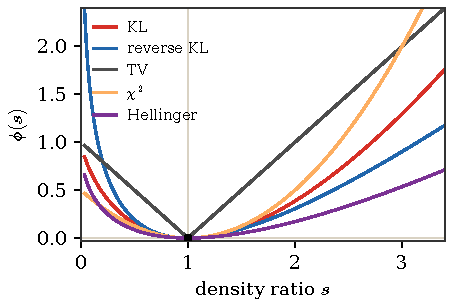
\includegraphics[width=.43\linewidth]{figures/dualnorms-phi-generators--generators.pdf} &
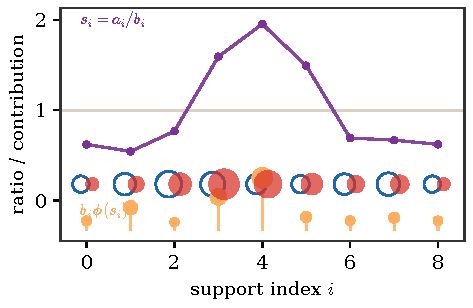
\includegraphics[width=.43\linewidth]{figures/dualnorms-phi-generators--ratio-penalties.pdf}
\end{tabular}
\caption{$\phi$-divergences through density ratios. The left panel shows normalized generators for common divergences as functions of $s=\d\alpha/\d\beta$; all curves vanish at $s=1$ up to affine normalization. The right panel shows the discrete formula $D_\phi(a|b)=\sum_i b_i\phi(a_i/b_i)$: hollow blue circles encode $b_i$, filled red circles encode $a_i$, the violet curve gives the ratios $a_i/b_i$, and orange lollipops show local KL-type contributions.}
\index{phi-divergence}% strictindex
\index{density!ratio}% strictindex
\label{fig:dualnorms-phi-generators}
\end{figure}

\begin{rem}[$\phi$-divergences versus Bregman divergences]
\index{phi-divergence}% strictindex
\index{Bregman!divergence}% strictindex
	Except for KL-type entropies, $\phi$-divergences should not be confused with Bregman divergences. A $\phi$-divergence compares measures pointwise through the density ratio $\d\alpha/\d\beta$ and is invariant under measurable changes of variables. A Bregman divergence is generated by a convex functional on a linear space and compares two points through first-order Taylor error. KL is special because the integral entropy $\alpha\mapsto\int \rho\log\rho$ produces a Bregman divergence whose density-ratio form is also a $\phi$-divergence.
\index{convex!function}% strictindex
\index{phi-divergence}% strictindex
\index{density!ratio}% strictindex
\end{rem}

\paragraph{Variational dual formula.}
\index{variational dual formula}% strictindex

The following formula turns a pointwise density-ratio penalty into a dual optimization problem over test functions. It is the analogue, for $\phi$-divergences, of the Kantorovich dual formula for transport costs.
\index{phi-divergence}% strictindex
\index{density!ratio}% strictindex
\index{dual!formula}% strictindex

\begin{proposition}[Dual expression]
	A $\phi$-divergence can be expressed using the Legendre transform
\index{Legendre transform}% strictindex
	\eq{
		\phi^{*,\geq 0}(s) \eqdef \usup{t \in \RR^+} st - \phi(t)
	}
	(notice that we restrict the function to the positive real)
	of $\phi$ as % (see also~\eqref{eq-legendre})
	\eql{\label{eq-dual-div}
		\Divergm_\phi(\al|\be) = \usup{f: \X \rightarrow \RR} \int_\X f(x) \d\al(x) - \int_\X \phi^{*,\geq 0}(f(x)) \d\be(x).
	}
	which equivalently reads that the Legendre transform of $\Divergm_\phi(\cdot|\be)$ reads
\index{Legendre transform}% strictindex
	\eql{\label{eq-legendre}
		\foralls f \in \Cc(\Xx), \quad
		\Divergm_\phi^*(f|\be) = \int_\X \phi^{*,\geq 0}(f(x)) \d\be(x).
	}
\end{proposition}

\begin{proof}
		We first consider the superlinear case $\phi'_\infty=+\infty$, so that $\Dd_\phi(\al|\be)=+\infty$ if $\al$ does not have a density $\rho \geq 0$ with respect to $\be$, $\d\al=\rho \d\be$. Thus the Legendre-Fenchel transform of $\Dd_\phi(\cdot|\be)$
	reads
	\begin{align*}
		\Dd_\phi^*(f|\be) &= \usup{\rho \geq 0} \int_\Xx f(x) \rho(x)\d\be(x) - \int_\Xx \phi(\rho(x)) \d\be(x)\\
			&= \int_\Xx \usup{\rho(x) \geq 0} \pa{ f(x) \rho(x) -\phi(\rho(x)) }\d\be(x)
		= \int_\Xx \phi^{*,\geq 0}(f(x)) \d\be(x).
	\end{align*}
		Fenchel--Moreau then gives the displayed dual expression. For a general entropy, the same argument is applied to the perspective with its recession term; the singular part is exactly encoded by the effective domain of $\phi^{*,\geq0}$.
	\end{proof}


%%%%%%%%%%%%%%%%%%%%%%%%%%%%%%%%%%%%%%%%%%%%%%%%%%%%%%%%%%%%%%%
\section{GANs via Duality}
\index{GAN}% strictindex


GANs fit naturally into the dual viewpoint: the discriminator is a parameterized potential and the generator moves a reference measure. This section first explains the original divergence-based GAN objective, then contrasts it with integral probability metrics such as MMD and Wasserstein distances.
\index{maximum mean discrepancy}% strictindex
\index{integral probability metric}% strictindex
\index{Wasserstein!distance}% strictindex
\index{reference!measure}% strictindex

The goal is to fit a generative parametric model $\al_\th = g_{\th,\sharp} \zeta$ to empirical data $\be = \frac{1}{m}\sum_{j} \de_{y_j}$, where $\zeta \in \Mm_+^1(\Zz)$ is a fixed density over the latent space and $g_\th : \Zz \rightarrow \Xx$ is the generator, often a neural network.

\paragraph{Divergence-based adversarial losses.}
\index{adversarial!loss}% strictindex

Any $\phi$-divergence can be written in adversarial form through the dual formula~\eqref{eq-dual-div}:
\index{phi-divergence}% strictindex
\index{dual!formula}% strictindex
\eq{
	\umin{\th} \Divergm_\phi(\al_\th|\be)
	= \umin{\th} \usup{\f} \int_\Xx f(x) \d\al_\th(x) - \Divergm_\phi^*(f|\be)
	= \umin{\th} \usup{\f} \int_\Xx f(g_\th(z)) \d\zeta(z) -
	\frac{1}{m}\sum_j \phi^*(f(y_j)).
}
Replacing the unrestricted potential $f$ by a neural network $f_\xi$ gives a saddle problem
\[
	\min_\theta\max_\xi
	\int_\Zz f_\xi(g_\theta(z))\d\zeta(z)
	-
	\frac1m\sum_j \phi^*(f_\xi(y_j)).
\]
The original vanilla GAN~\cite{GAN} is this construction for the Jensen--Shannon generator discussed above,
\[
	\phi_{\JS}(s)=s\log s-(s+1)\log\frac{s+1}{2},
	\qquad
	\phi_{\JS}^*(u)=-\log(2-e^u),\quad u<\log2,
\]
up to affine normalizations and the usual reparametrization of the potential by a discriminator with values in $(0,1)$. In practice the min--max problem is solved by alternating stochastic gradient descent/ascent on $(\theta,\xi)$. Unlike the convex-concave variational formula, the neural parametrization is non-convex in $\theta$ and non-concave in $\xi$, which explains the instability and mode-collapse pathologies of divergence-based GAN training. These losses estimate density ratios, which is statistically meaningful when the measures overlap but can saturate when the model and data are mutually singular; for example, the Jensen--Shannon divergence is maximal for disjoint supports.
\index{stochastic!gradient}% strictindex
\index{Jensen-Shannon divergence}% strictindex
\index{density!ratio}% strictindex

\paragraph{Dual norms and integral probability metrics.}
\index{dual!norm}% strictindex
\index{integral probability metric}% strictindex

Instead of a density-ratio divergence, one can minimize a dual norm~\eqref{eq-dual-norm-cont}, also called an integral probability metric,
\index{density!ratio}% strictindex
\eq{
	\umin{\th} \norm{\al_\th - \be}_B
	= \umin{\th}
	\usup{\f \in B} \int_{\X} \f(x) \d(\al_\th-\be)(x)
	= \umin{\th}
	\usup{\f \in B} \int_{\Zz} \f( g_\th(z)) \d\zeta - \frac{1}{m} \sum_j f(y_j).
}
MMD-GANs take $B$ to be a unit ball in an RKHS~\cite{MMD-GAN}; Wasserstein GANs take $B$ to be a Lipschitz ball, following Kantorovich--Rubinstein duality~\cite{WassersteinGAN,FrognerNIPS}. The advantage of such choices is topological: for bounded continuous RKHS balls, or for bounded Lipschitz balls on compact spaces, the resulting objective is weak-* continuous. It can therefore compare singular empirical and generated measures through test functions, instead of requiring pointwise density ratios. The price is that the discriminator class must be controlled geometrically, either by a kernel norm, a Lipschitz constraint or a related regularization.
\index{kernel!norm}% strictindex
\index{RKHS}% strictindex
\index{maximum mean discrepancy}% strictindex
\index{Kantorovich-Rubinstein!duality}% strictindex
\index{discriminator class}% strictindex
\index{density!ratio}% strictindex
%

\begin{rem}[Weight clipping is only a proxy]
	Wasserstein GANs originally used weight clipping, constraining $\norm{\xi}_\infty \leq 1$ as a proxy for enforcing $\f_\xi \in B = \enscond{f}{\Lip(f) \leq 1}$. This parameter set is both smaller than the true Lipschitz ball and non-convex, so clipping should be understood as a practical heuristic rather than a faithful implementation of the Kantorovich--Rubinstein dual constraint.
\end{rem}
